% !TeX root = ../main.tex
% Add the above to each chapter to make compiling the PDF easier in some editors.

\chapter{Introduction}\label{chapter:introduction}

\section{General Overview} 

In many clinical settings, obtaining intravenous access is an essential and routinely performed operation in medical procedures like blood sampling, collection, donation and intravenous therapy where some of these operations include a cannulation as well.
Today, venepuncture procedures are conducted almost exclusively by trained clinical personnel. In this approach, the operator visually locates or palpates for a suitable vein and then introduces a cannula aiming to reach the center of the vein. The standard practice of using surface anatomy to identify vessels before cannulation is based on the presumed location of the vessel and the identification of skin anatomical landmarks. Oftentimes, however, it is difficult to find a suitable cannulation site, particularly in patients with small veins, dark skin, or a high body weight. When a vein is identified, it may also be difficult to estimate its depth or to accurately place the cannula if the vein moves. For these reasons, successful venepuncture depends heavily on the patient's physiological characteristics and the operator's experience and skill.

Depending on the cannulation site, manual techniques for peripheral vascular access have an overall success rate of 70 to 95\% \parencite{clinicalPredi}, \parencite{comlicationsVeni1}. The success rate can decrease below 50\% in difficult populations, including paediatric, geriatric, and chronically-ill patients \parencite{comlicationsVeni2} . On average, difficult
patients require three needle stick attempts per vessel, and the incidence of complications increases when more than three attempts are made by the same operator. venepuncture injuries due to multiple failed attempts significantly increase the likelihood of bruising, internal bleeding, acute pain, accidental puncture of nerves or arteries, and delays in medical treatment. The inaccurate placement of a peripheral catheter increases the chance of extravasation and tissue damage, and repeated failures may necessitate a switch to riskier and more costly interventions such as central venous access \parencite{clinicalPredi}.  


This solution utilizes a near-infrared light source to image the oxygenated haemoglobin in red blood cells, enabling a NIR-camera to capture a clear image of the superficial veins in real-time. 

\section{Complications Associated with Venepuncture}

Several complications can arise during the peripheral venous access, the most common ones are described below and listed approximately in order of their frequency of occurrence \parencite{comlicationsVeni}, \parencite{roboVenipuncture}.

\subsubsection{Pain}
Needle pain is commonly reported by patients as the worst of all healthcare issues and might result in stress symptoms, tension, and onset of needle phobia. Avoidance of healthcare visits, for example for ordinary blood tests or immunization, is strongly related to the fear of needle pain. pain is even more feared when multiple needle insertions are needed, as an example, in difficult populations or when complications such as hematoma and nerve puncture occur.

\subsubsection{Failure to Access the Vein}
Wrong needle placing, incorrect angle of penetration, inadequate skin traction, or vein collapse can cause a failed attempt at gaining access to the vein. In this situation, many insertions are needed, either on the same place or, if the vein or the skin is compromised, at a another one.

\subsubsection{Hematoma}
Hematomas are one of the most common complications associated with peripheral venous access and are usually formed when blood leaks out of the vessel into the surrounding tissues. Hematomas are caused by a damage to the wall of the vessel through puncture and can be noticed under the skin as a massive bruise. The bruise causes discomfort and pain and can cause further complications. Hematomas are mainly common in children and elderly patients. In children, small vessels can easily be damaged or rupture if the needle tip punctures the posterior wall.
In elderly patients, vessels become weak because of hardening of the vessel wall, which will increase the chance of vein rupture. 

%\hfill
%\begin {center}
%\includegraphics{logos/hematoma.jpg}
%Image 1 Hematoma on donator's arm three days after a needle came out of his vein during a plateletpheresis donation at a Red Cross donation center in Liverpool, NY. 
%\end {center}

\subsubsection{Unintended Arterial Puncture}
Sometimes, it may be difficult to differentiate arteries from veins. Usually, healthcare workers avoid accidental arterial puncture by palpating the vein carefully to make sure that there's no detectable pulse before inserting the needle. 
However, it is harder to detect palpation, and arteries can be easily mistaken as veins in young children and obese patients. When an accidental arterial puncture occurs and is not identified, the delivery of intravenous fluids such as medicines into the arterial circulation can cause serious complications \parencite{comlicationsVeni3}.

\subsubsection{Peripheral Nerve Damage}
Accidental puncture of nerves is rare but can happen when the nerves are located near a vessel \parencite{comlicationsVeni4}. It occurs most often if the needle is not accurately inserted in the vessel, or if the vessel moves away from the puncturing point after penetrating the skin and causes the needle to puncture an adjacent nerve. Nerves in the antecubital fossa area lie just beneath, and near the veins making them vulnerable to injury \parencite{comlicationsVeni4}.
The best site for venepuncture of superficial veins of the upper limbs is the median cubital vein which lies over the cubital fossa and serves as a connection between the cephalic and basilic veins. That makes the median nerve particularly prone to accidental puncture, as it is located just after the basilic vein in the antecubital fossa and can lead to acute pain, numbness, or even, in rare cases, temporary paralysis in the region of the cannulation site.

\subsubsection{Phlebitis}
Inflammation of the veins, which can occur because of an accidental puncture of the posterior vessel wall or the rupture of the side walls during puncturing or cannulation insertion. mainly when delivering medications, movements of the needle or catheter can irritate the vessel. Phlebitis can be recognized by some usual symptoms like pain, swelling, redness, and tenderness and it can produce extreme medical complications if not detected. 


\section{Background: Infrared Radiation}
\subsubsection{Light Spectrum}
The light or electromagnetic spectrum is a range of all types of EM radiation and it describes all the wavelengths of light. 
The EM spectrum, as shown in \autoref{fig:electromagneticRadiation} \parencite{electromagnetic}, is generally divided into seven regions, ordered by decreasing wavelength and increasing energy and frequency: radio waves, microwaves, infrared (IR), visible light, ultraviolet (UV), X-rays and gamma rays. 


\begin{figure}[H]
\centering
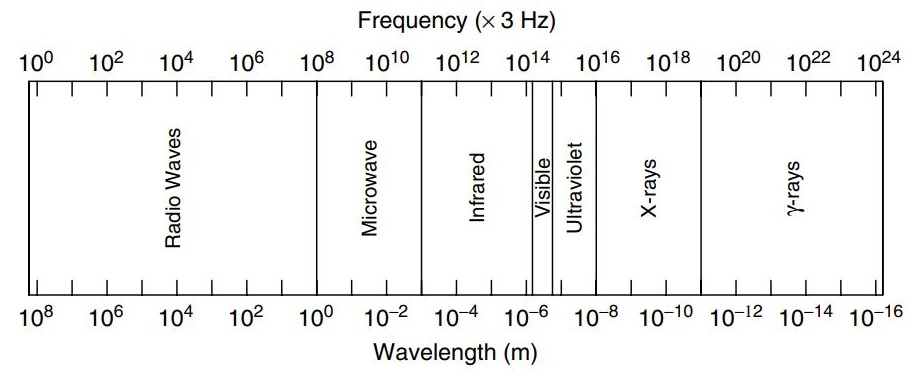
\includegraphics[scale=0.5]{figures/electromagneticRadiation.JPG}
\caption[The electromagnetic radiation spectrum]{The electromagnetic radiation spectrum.}\label{fig:electromagneticRadiation}
\end{figure}



\subsubsection{Infrared Radiation}
Infrared radiation is a region of the EM radiation spectrum where wavelengths range from about 700 nm to 1 mm. Infrared waves are longer than those of visible light, but shorter than those of radio waves. 
Infrared light is invisible to the human eye, but longer infrared waves can be sensed as heat and it shares some characteristics with visible light, infrared light can be focused, reflected and polarized.
Based on wavelength, infrared can be divided into multiple spectral regions near-, mid- and far-infrared where the boundaries between them are not agreed upon and can vary.
 

The near-IR band contains the range of wavelengths closest to the red end of the visible light spectrum. It consists of the wavelengths from 700 nm to 1,300 nm. This group consists of the longest wavelengths and shortest frequencies, and it produces the least heat.

The intermediate IR band, also called the mid-IR band, covers wavelengths ranging from 1,300 nm to 3,000 nm. 
Wavelengths in the far-IR band, which are closest to microwaves, extend from 3,000 nm to 1 mm. This group consists of the shortest wavelengths and longest frequencies, and it produces the most heat.


\section{Previous Findings}

Due of the challenges associated with venepuncture, development of imaging technology has become essential. In this area, two non-invasive methods are commonly used: ultrasound (US) signals and near-infrared (NIR) light. The focus in this work is on NIR imaging.
In this section, previous findings are described and discussed as well as the difference between US and NIR imaging techniques and reasons for choosing NIR over US imaging.

\subsection{Ultrasound vs. Near-Infrared Imaging}

\subsubsection{Ultrasound Imaging}
Using US can provide visual information of the size and depth of blood vessels, which could enable insertion of the needle in real time. In comparison with light waves (including NIR waves), acoustic waves can penetrate deeper into human tissue, allowing both superficial and deep tissues to be visualized. 

The use of US imaging has shown potential to improve the success of cannula insertion and Reducing complications. They are appropriate for imaging vascular structures and surrounding areas, usually, using 2D imaging, Doppler colour flow, and Spectral Doppler. The main feature of the US over NIR light imaging is the ability to image tissue laying far beneath the penetration limits of NIR light. 

Although, the size and cost of US imaging devices have been reduced in recent years, NIR imaging is more effective in terms of ease-of-use and has way shorter learning curve. Using the US, the operator must be able to interpret the two-dimensional images of the vessels and distinguish them from surrounding structures. However, this technique requires a high coordination between hand and eye to scan and insert the needle simultaneously depending on the live images. Though the use of the colour Doppler can confirm the presence and direction of blood flow, it requires an understanding of the mechanisms of Doppler image generation as well as performing the 3D task of placing a needle or catheter into a vessel based on 2D images and not to mention the fact that the transducer must stay in contact with the examined person’s skin all the time during examination.

Additionally, to visualize the needle inside the image, the operator holds the transducer parallel with the vessel then align the needle parallel to the imaging plane and the vessel and maintain the needle in the plane as it is inserted into the vessel. Deviations of 1 or 2 mm will cause the needle to disappear from the image. If the vessel rolls far from the image plane, it can also become invisible. Patient movement will likewise cause significant image distortions and make it difficult to maintain the visibility of needle and the vessel. Thus, it's far very hard to visualize the needle as it punctures the vessel and the operator is left to infer the needle motion primarily based on the motion of the vessel.

\subsubsection{Near-Infrared Imaging}

NIR involves the projection of light on the skin. NIR light operates typically within the wavelength range from 700 to 1300 nm. Compared to visible light, NIR waves penetrate more deeply into scattering tissues because of low absorption and scattering rates of light through skin tissues at NIR wavelengths. NIR can allow monitoring of vessels up to 3 mm under the skin and thus, provide good contrast and visualization.

NIR imaging depends on the fact that NIR can penetrate the skin and then haemoglobin in the veins absorbs it, structuring an image of the vascular pattern which is invisible to human eye but can be captured by an NIR camera. The images from the camera are then processed and displayed in real time either on a screen or projected back onto the patient’s skin and thus, providing a good visualization of the veins structure. NIR transmitters must not make any contact with the skin and are, therefore, easier to use compared to US transducers. Moreover, because the images are acquired in a top-down manner, difficulties related to the vessel or the needle disappearing from the image are avoided.

However, NIR imaging have some limitations. The major limitation is the maximum possible imaging depth. All vessels laying more than 3 mm in depth cannot be visualized due to penetration limitation of the NIR light. That makes NIR imaging less usable for patients with special skin conditions like skin diseases or scars that increase the skin thickness or for patients with high body weight.

Another limitation of the NIR imaging is that the 2D images don’t provide information about the depth of the vessel and thus cannot inform the operator about whether the needle has penetrated the vessel and punctured the posterior vessel wall for example. This is important because many of the adverse events that occur during cannulation, including poor sample collection and hematoma occur mostly due to posterior wall puncture.
Lastly, it could be difficult to differentiate arteries from veins using NIR imaging, especially in obese patients or children where the pulse in the arteries is more difficult to be identified via palpation. 

\subsubsection{Conclusion}
Both US and NIR imaging techniques have features and limitations and depending on problem specifications, one can choose the suitable technique. NIR technique is better for a simple 2D imaging and it comes with a feature that no contact with the skin is needed and it is easier to use especially for relatively untrained personal, on the other side, US technique is preferred for more complex situations as it offers a 3D visualization of the veins pattern and it can penetrate more deeply than NIR but it requires eye-hand-coordination skills and a founded knowledge about Doppler image generation. We focused on the NIR imaging, due to the shorter learning curve and ease-of-use of it and because of the fact that the main focus is to develop a simple low-cost vein-viewing mobile system.


\subsection{Studies and Products}

In this area, a lot of studies have taken place and a lot of products have been developed in the last years. While some of the prototypes and products developed give promising results, they are either too big to be handheld and portable or too expensive because of the advanced technologies utilized in them. Below is a brief list of studies and methods used in some products.

\subsubsection{Studies}

The shared drawback between the studies in this field ,as in \parencite{study1} and \parencite{study2}, is that a computer must be used to process the data coming
from the NIR camera. Which lacks portability as it can just run on a computer which is not as portable as mobile phone. More importantly it lacks usability because it’s hard to use a
computer as AIR aiding device in such case, as one needs to look at the computer screen
and the examined limb at the same time. Which is not the case when using a mobile
smartphone just above the examination area.

\subsubsection{Dedicated Devices}
Dedicated devices for viewing and locating veins have been launched in the market and a lot of them use NIR light and NIR cameras. While some of them show the results as projected light directly on the examined limb as hologram, others show them on a screen. Although they seem to give excellent results in terms of accuracy and performance, they include advanced and expensive hardware which makes them unaffordable for every healthcare facility.
\subsubsection{USB NIR Cameras}
An NIR camera which can be connected to a normal computer via USB, where a windows application shows a real-time video of the limb with contrast of the superficial veins. Although the result seems to be fair, but as in the dedicated devices, it suffers from the lack of portability and usability.

\subsubsection{NIR Transilluminators}

Usually devices with plastic ring-shaped head where high power NIR as well as red visible light
emitters are placed. Results are examined then with naked eye. Results seem to be adequate,
when examining healthy light skin-color people, but results are going to be inadequate when examining dark skin-color people or those with some special skin conditions because the used technique is strongly dependant on such factors.




 